\section{Introducción y objetivos}


\begin{frame}[c]{Motivación}

    El comportamiento de las enfermedades infecciosas es especialmente relevante en países menos desarrollados, pues sufren consecuencias más graves.
    \\~\\
    Los modelos matemáticos en epidemiología ayudan a comprender los mecanismos que intervienen en la propagación de las enfermedades y sugerir mecanismos para su control.

\end{frame}


\begin{frame}{Objetivos}

    \begin{itemize}
        \item Marcados al inicio:

        \pause
        \begin{itemize}
            \item Descripción y estudio de modelos discretos en epidemiología.
            \pause
            \item Visualización del comportamiento de los modelos.
            \pause
            \item Desarrollo de una página web.
        \end{itemize}
        
        \pause
        \item Adicionales:

        \pause
        \begin{itemize}
            \item Descripción y estudio de modelos continuos en epidemiología.
            \pause
            \item Ajuste de datos.
            \pause
            \item Ajuste de datos reales.
        \end{itemize}
    \end{itemize}

\end{frame}


%%%%%%%%%%%%%%%%%%%%%%%%%%%%%%%%%%%%%%%%%%


\section{Herramientas básicas}


\begin{frame}{Ecuaciones en diferencias}
    
    \begin{textblock*}{12cm}(0.5cm,1cm)
	
        \begin{block}{Ecuación en diferencias}
            Se define una ecuación en diferencias de orden $k$, con $k\geq 1$, como una ecuación en la que intervienen un número fijo de términos consecutivos de una sucesión:

            \begin{equation}
            F(n,X_n, X_{n+1}, \cdots , X_{n+k}) = 0, \quad \forall n\in\mathbb{N},
            \end{equation}
            
            
            donde $F$ es una función de $k+2$ variables en la forma $F:\mathbb{N}\times I^{k+1}\rightarrow \mathbb{R}$, con $I$ un intervalo con al menos dos puntos, $k$ indica el número de términos necesarios para generar el siguiente y donde la sucesión $\{X_n\}_{n\geq 0}$ es la incógnita.
        \end{block}
        
    \end{textblock*}

\end{frame}


\begin{frame}{Sistema de ecuaciones en diferencias}

    \begin{textblock*}{12cm}(0.5cm,1cm)
	
        \begin{block}{Sistema de ecuaciones en diferencias}
            Se define un sistema de $m$ ecuaciones en diferencias como un conjunto de $m$ ecuaciones en diferencias a resolver.

            \begin{equation}
            \begin{cases}
            X_{n+k}^1 = \Phi_1(n, X_n^1, \cdots , X_{n+k-1}^1, X_{n}^2, \cdots , X_{n+k-1}^2, \cdots , X_{n}^m, \cdots X_{n+k-1}^m) \\
            \cdots \\
            X_{n+k}^m = \Phi_m(n, X_n^1, \cdots , X_{n+k-1}^1, X_{n}^2, \cdots , X_{n+k-1}^2, \cdots , X_{n}^m, \cdots X_{n+k-1}^m)
            \end{cases}
            \end{equation}

            Donde $\Phi_i : \mathbb{N}\times D \rightarrow D$, con $D\subset \mathbb{R}^{mk}$ para todo $i=1,\cdots , m$.

            Renombrando, podemos expresar el conjunto de sucesiones como:

            \begin{equation}
            X_n = (X_{n}^1, X_{n}^2, \cdots , X_{n}^m)^{T}
            \end{equation}

            luego el sistema de ecuaciones resultaría:

            \begin{equation}
            \label{def_sist_ec}
            X_{n+k} = \Phi (n, X_n, \cdots , X_{n+k-1})
            \end{equation}


            donde $\Phi : D \rightarrow D$, con $D$ siendo el dominio de la función $\Phi$, y por tanto $D\subset \mathbb{N}\times\mathbb{R}^k$ y con $\Phi = (\Phi_1, \cdots , \Phi_m)$.
        \end{block}
        
    \end{textblock*}


\end{frame}


\begin{frame}{Puntos fijos}

    \begin{textblock*}{12cm}(0.5cm,1cm)
        \begin{block}{Puntos fijos}
            Sea $D\subset \mathbb{R}^m$ y $\Phi :D\rightarrow D$ una función continua. Entonces un vector $X^* \in D$ se dice que es un \textbf{punto de equilibrio} de un sistema de ecuaciones en diferencias si

            $$X^* = \Phi (X^*),\quad X^* \in D.$$

        \end{block}  
        
        Se suele decir que los puntos fijos son soluciones independendientes del tiempo.
    \end{textblock*}



\end{frame}


\begin{frame}{Conceptos fundamentales (I)}

    \begin{block}{Epidemia}
        Las epidemias son brotes espontáneos de una enfermedad o situaciones endémicas, en las que la enfermedad está siempre presente.
    \end{block}  

\end{frame}



\begin{frame}{Conceptos fundamentales (II)}

    \begin{block}{Individuos susceptibles}
        Los individuos \textbf{susceptibles}, que denotamos $S_n$, son aquellos que pueden infectarse con la enfermedad pero aún no lo han hecho en el momento $n$.
    \end{block}  

    \pause

    \begin{block}{Individuos infectados}
        Los individuos \textbf{infectados}, a los que denotamos $I_n$, son las personas infectadas en el instante $n$ por la enfermedad y pueden contagiar la enfermedad a los individuos susceptibles.
    \end{block}  

    \pause

    \begin{block}{Individuos recuperados}
        Los individuos \textbf{recuperados}, que denotamos $R_n$, son los individuos que han estado infectados y ya no contagian la enfermedad ni pueden volver a infectarse.
        Los individuos recuperados hacen referencia a los individuos inmunizados, aislados, recuperados o fallecidos.
    \end{block}  


\end{frame}


\begin{frame}{Suposiciones base}

    En todos los modelos se parte de realizan las siguientes suposiciones:

    \begin{itemize}
        \item La población se mezcla de manera homogénea, es decir, todos los individuos tienen la misma probabilidad de interactuar entre ellos y contraer la enfermedad.
        \item El total de la población es constante y lo denotaremos por $N$.
    \end{itemize}

\end{frame}


%%%%%%%%%%%%%%%%%%%%%%%%%%%%%%%%%%%%%%%%%%


\section{Modelos discretos en epidemiología}


\subsection{Modelo SI}


\begin{frame}{Modelo SI (I)}

    \begin{block}{Modelo SI}

        \begin{equation}
        \label{eqn: SI}
        \begin{aligned}
        S_{n+1}=S_n\left( 1-\frac{\alpha\Delta t}{N}I_n\right) \\
        I_{n+1}=I_n\left( 1+\frac{\alpha\Delta t}{N}S_n\right)
        \end{aligned}
        \end{equation}

        Con condiciones iniciales $S_0>0$, $I_0>0$ y $S_0+I_0=N$.
        

    \end{block}  

    %\begin{itemize}
    %    \item $S_n$: número de individuos susceptibles en el instante $t_n$.
    %    \item $I_n$: número de individuos infectados en ese instante.
    %    \item $\Delta t$: tiempo transcurrido entre dos instantes $t_{n+1}-t_n$. 
    %    \item $\alpha$ es la tasa de contacto; es decir, el número medio de individuos con los que un infectado tiene suficiente contacto para contagiarlo en un intervalo de tiempo.
    %\end{itemize}

\end{frame}

\begin{frame}{Modelo SI (II)}
 
    \begin{proposition}
        Las soluciones de las ecuaciones \eqref{eqn: SI} son positivas si y solo si $\alpha\Delta t \leq 1$.
    \end{proposition}
    
    \pause

    \begin{lema}
        $S_n$ es monótonamente decreciente e $I_n$ es monótonamente creciente.
    \end{lema}

    \pause

    Los únicos puntos de equilibrio posibles son: $(S^*,I^*)=(0,N)$ y $(S^*,I^*)=(N,0)$.
    
    El sistema debe converger a $(S^*,I^*)=(0,N)$.



\end{frame}

\begin{frame}{Modelo SI (III)}
    \begin{figure}
        \begin{center}
        \caption{Gráfica del modelo SI discreto, en una población total de $100$ individuos, con valores iniciales $S_0=99, I_0 = 1, \alpha = 0.1, T_0 = 0, T = 100$.}
        \includegraphics[scale=0.6]{graficaSI}
        \end{center}
    \end{figure}
\end{frame}


\begin{frame}{Modelo SI (IV)}
    \begin{figure}
        \begin{center}
        \caption{Gráfica del modelo SI, representando el número de infectados según el número de individuos susceptibles, en una población total de $100$ individuos, con valores iniciales $S_0=99, I_0 = 1, \alpha = 0.1, T_0 = 0, T = 100$.}
        \label{fig: SI_IsobreS}
        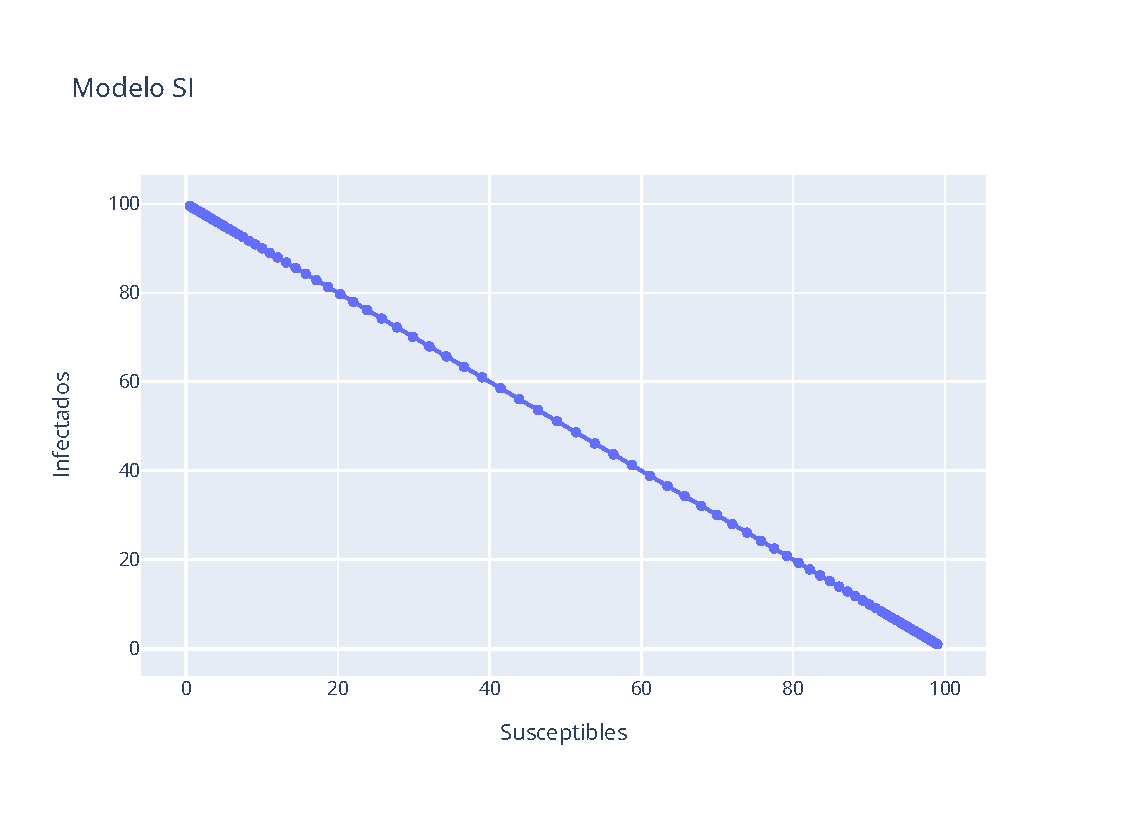
\includegraphics[scale=0.5]{SI_IsobreS}
        \end{center}
        \end{figure}
\end{frame}


\subsection{Modelo SIR}


\begin{frame}{Modelo SIR (I)}

    \begin{block}{Modelo SIR}
        \begin{equation}
        \label{eqn: SIR_modelo}
        \begin{aligned}
        S_{n+1} = & S_n \left(1-\frac{\alpha\Delta t}{N} I_n \right) \\
        I_{n+1} = & I_n \left( 1-\gamma \Delta t + \frac{\alpha\Delta t}{N} S_n \right) \\
        R_{n+1} = & R_n + \gamma \Delta t I_n
        \end{aligned}
        \end{equation}
        
        Con condiciones iniciales $S_0>0$, $I_0>0$, $R_0\geq 0$, satisfaciendo $S_0+I_0+R_0=N$.
    \end{block}
\end{frame}


\begin{frame}{Modelo SIR (II)}
    \begin{proposition}
        Las soluciones a este sistema discreto son positivas para cualquier valor de las condiciones iniciales si, y solo si:
        $$\max{\big\{\gamma\Delta t, \alpha\Delta t\big\} } \leq 1,$$
        
        o equivalentemente  
        $\min{\bigg\{ \frac{1}{\gamma}, \frac{1}{\alpha} \bigg\} } \geq \Delta t.$
        
        \end{proposition}

        \pause 

        \begin{lema}
            $S_n$ es estrictamente decreciente y $R_n$ es estrictamentre creciente.
        \end{lema}

        \pause

        \begin{definition}
            Definimos el número básico reproductivo como la constante 
            $$\mathcal{R}_{SIR}=\frac{S_0 \alpha}{N\gamma }.$$
        \end{definition}


\end{frame}

\begin{frame}{Modelo SIR (III)}
    \begin{figure}
        \begin{center}
        \caption{Gráfica del modelo SIR, en una población total de $100$ individuos, con valores iniciales $S_0=99, I_0 = 1, R_0 = 0, \alpha = 0.1, \gamma = 0.01, T_0 = 0, T = 300$.}
        \includegraphics[scale=0.6]{graficaSIR}
        \end{center}
    \end{figure}
\end{frame}

\begin{frame}{Modelo SIR (IV)}

    \begin{columns}
        \column{0.5\textwidth}
        \begin{minipage}[c][0.4\textheight][c]{\linewidth}
          \centering
          \includegraphics[width=1.2\linewidth]{SIR_IsobreS}
        \end{minipage}
        \begin{minipage}[c][0.4\textheight][c]{\linewidth}
            \begin{enumerate}
                \item Individuos infectados en función de los susceptibles.
                \item Individuos recuperados en función de los susceptibles.
                \item Individuos recuperados en función de los infectados.
            \end{enumerate}
          
        \end{minipage}
        \column{0.5\textwidth}
        \begin{minipage}[c][0.4\textheight][c]{\linewidth}
            \centering
            \includegraphics[width=1.2\linewidth]{SIR_RsobreS}
        \end{minipage}
        \begin{minipage}[c][0.4\textheight][c]{\linewidth}
          \centering
          \includegraphics[width=1.2\linewidth]{SIR_RsobreI}
        \end{minipage}
        \end{columns}

\end{frame}


\subsection{Modelo SIS}


\begin{frame}{Modelo SIS (I)}
    \begin{block}{Modelo SIS}
        \begin{equation}
            \label{eqn: modelo_SIS}
            \begin{aligned}
            S_{n+1} & = S_n \left(1-\frac{\alpha\Delta t}{N} I_n \right) + \gamma \Delta t I_n \\
            I_{n+1} & = I_n \left( 1-\gamma \Delta t + \frac{\alpha\Delta t}{N} S_n \right)
            \end{aligned}
            \end{equation}
            
            Con condiciones iniciales $S_0>0$, $I_0>0$ cumpliendo $S_0+I_0=N$.
    \end{block}
\end{frame}


\begin{frame}{Modelo SIS (II)}

    \begin{proposition}
        Las soluciones de \eqref{eqn: modelo_SIS} siempre son positivas si, y solo si:
        
        $$\gamma \Delta t \leq 1 $$ y $$\alpha\Delta t< \left( 1+\sqrt{\gamma \Delta t} \right)^2$$
        
    \end{proposition}

    \begin{lema}
        Los puntos de equilibrio de \eqref{eqn: modelo_SIS} son o bien $(S^*,I^*)=(N,0)$, o bien $(S^*,I^*)=(\frac{N\gamma}{\alpha}, N-\frac{N\gamma}{\alpha})$.
    \end{lema}

    \begin{definition}
        El número básico reproductivo se define como 
        $$\mathcal{R}_{SIS}=\frac{\alpha}{\gamma}.$$
    \end{definition}
\end{frame}


\begin{frame}{Modelo SIS (III)}


    \begin{figure}
        \begin{center}
        \caption{Gráfica del modelo SIS, en una población total de $100$ individuos, con valores iniciales $S_0=95, I_0 = 5, \alpha = 0.1, \gamma=0.01, T_0 = 0, T = 150$.}
        \includegraphics[scale=0.5]{SIS_modelo}
        \end{center}
    \end{figure}

\end{frame}



\subsection{Modelos multipoblacionales}


\begin{frame}{Modelos multipoblacionales}

\end{frame}


%%%%%%%%%%%%%%%%%%%%%%%%%%%%%%%%%%%%%%%%%%


\section{Modelos continuos en epidemiología}


\subsection{Modelo SI}


\begin{frame}{Modelo SI}

\end{frame}


\subsection{Modelo SIS}


\begin{frame}{Modelo SIS}

\end{frame}


\subsection{Modelo SIR}


\begin{frame}{Modelo SIR}

\end{frame}


%%%%%%%%%%%%%%%%%%%%%%%%%%%%%%%%%%%%%%%%%%


\section{Desarrollo del software: análisis y diseño}


\subsection{Análisis y diseño}


\begin{frame}{}

\end{frame}


\begin{frame}{Ajuste de datos}

\end{frame}


\subsection{Demostración}


\begin{frame}{Demostración de uso}

    \href{run:/home/mapachana/2022-06-23 19-38-25.mkv}{Click for video}

\end{frame}


\subsection{Datos reales}


\begin{frame}{El Covid-19 en España}

\end{frame}


\begin{frame}{El VIH en Baleares}

\end{frame}


%%%%%%%%%%%%%%%%%%%%%%%%%%%%%%%%%%%%%%%%%%


\section{Conclusiones}


\begin{frame}{Conclusiones}

\end{frame}


%%%%%%%%%%%%%%%%%%%%%%%%%%%%%%%%%%%%%%%%%%

\begin{frame}{Referencias}
    \bibliography{../redaccion_tfg/bib/library.bib}
    \bibliographystyle{plain}
\end{frame}


\begin{frame}[c]{}
\begin{center}
\large{\textbf{Gracias por su atención.}}
\end{center}
\end{frame}
